\documentclass[10pt]{article}  

%%%%%%%% PREÁMBULO %%%%%%%%%%%%
\title{Reporte de Laboratorio}
\usepackage[spanish]{babel} %Indica que escribiermos en español
\usepackage[utf8]{inputenc} %Indica qué codificación se está usando ISO-8859-1(latin1)  o utf8  
\usepackage{amsmath} % Comandos extras para matemáticas (cajas para ecuaciones,
% etc)
\usepackage{amssymb} % Simbolos matematicos (por lo tanto)
\usepackage{longtable} %agregadom para hacer tablas
\usepackage{xltabular}
\usepackage{tabularray}
\usepackage{graphicx} % Incluir imágenes en LaTeX
\usepackage{color} % Para colorear texto
\usepackage{subfigure} % subfiguras
\usepackage{float} %Podemos usar el especificador [H] en las figuras para que se
% queden donde queramos
\usepackage{capt-of} % Permite usar etiquetas fuera de elementos flotantes
% (etiquetas de figuras)
\usepackage{sidecap} % Para poner el texto de las imágenes al lado
	\sidecaptionvpos{figure}{c} % Para que el texto se alinie al centro vertical
\usepackage{caption} % Para poder quitar numeracion de figuras
\usepackage{commath} % funcionalidades extras para diferenciales, integrales,
% etc (\od, \dif, etc)
\usepackage{cancel} % para cancelar expresiones (\cancelto{0}{x})
 
\usepackage{anysize} 					% Para personalizar el ancho de  los márgenes
\marginsize{2cm}{2cm}{2cm}{2cm} % Izquierda, derecha, arriba, abajo

\usepackage{appendix}
\renewcommand{\appendixname}{Apéndices}
\renewcommand{\appendixtocname}{Apéndices}
\renewcommand{\appendixpagename}{Apéndices} 
% Para que las referencias sean hipervínculos a las figuras o ecuaciones y
% aparezcan en color
\usepackage[colorlinks=true,plainpages=true,citecolor=blue,linkcolor=blue]{hyperref}
%\usepackage{hyperref} 
% Para agregar encabezado y pie de página
\usepackage{fancyhdr} 
\pagestyle{fancy}
\fancyhf{}
\fancyhead[L]{\footnotesize UNI} %encabezado izquierda
\fancyhead[R]{\footnotesize Fac. de Ciencias}   % dereecha
\fancyfoot[R]{\footnotesize Informe}  % Pie derecha
\fancyfoot[C]{\thepage}  % centro
\fancyfoot[L]{\footnotesize Informe de Laboratorio.}  %izquierda
\renewcommand{\footrulewidth}{0.4pt}


\usepackage{listings} % Para usar código fuente
\definecolor{dkgreen}{rgb}{0,0.6,0} % Definimos colores para usar en el código
\definecolor{gray}{rgb}{0.5,0.5,0.5} 
% configuración para el lenguaje que queramos utilizar
\lstset{language=Matlab,
   keywords={break,case,catch,continue,else,elseif,end,for,function,
      global,if,otherwise,persistent,return,switch,try,while},
   basicstyle=\ttfamily,
   keywordstyle=\color{blue},
   commentstyle=\color{red},
   stringstyle=\color{dkgreen},
   numbers=left,
   numberstyle=\tiny\color{gray},
   stepnumber=1,
   numbersep=10pt,
   backgroundcolor=\color{white},
   tabsize=4,
   showspaces=false,
   showstringspaces=false}

\newcommand{\sen}{\operatorname{\sen}}	% Definimos el comando \sen para el seno
%en español

\title{Plantilla para Reportes IMEC-UTB}
% Basada en la plantilla para reportes UPIITA de  Overleaf

%%%%%%%% TERMINA PREÁMBULO %%%%%%%%%%%%

\begin{document}

%%%%%%%%%%%%%%%%%%%%%%%%%%%%%%%%%% PORTADA %%%%%%%%%%%%%%%%%%%%%%%%%%%%%%%%%%%%%%%%%%%%
																					%%%
\begin{center}																		%%%
\newcommand{\HRule}{\rule{\linewidth}{0.5mm}}									%%%\left
 																					%%%

\hspace{0.9cm}

\textsc{\huge Universidad Nacional de Ingeniería }\\[0.8cm]
			
\textsc{\LARGE Facultad de Ciencias}

\vspace{0.5cm}

\textsc{\Large Escuela profesional de Química}

\vspace{0.6cm}



\includegraphics[scale = 0.15]{Imagenes/UNI.png}
	
\vspace*{0.6cm}							

\begin{minipage}{0.9\textwidth} 
\begin{center}																					%%%
\textsc{\LARGE  Laboratorio de Química BQU01\\[0.3cm] Sección A }
\end{center}
\end{minipage}\\[0.3cm]
%%%
    																				%%%
 			\vspace*{0.4cm}																		%%%
																					%%%
\HRule \\[0.5cm]																	%%%
{ \huge \bfseries Reporte 03: Termoquímica}\\[0.3cm]	%%%
 																					%%%
\HRule \\[0.9cm]																	%%%
 																				%%%
																					%%%
\begin{minipage}{0.46\textwidth}													%%%
\begin{flushleft} \large															%%%

% Aqui a continuación pongan los nombres de los integrantes
\emph{El grupo conformado por:}\\	
Llactahuaman Quispe Benjamin\\
20232268G \\
\vspace{2mm}
 Cortez Núñez Christian\\
 20232203B\\
\vspace{2mm}
 Jiménez Contreras Juan\\
 20230468I\\
 

%%%
			%\vspace*{2cm}	
            													%%%
										 						%%%
\end{flushleft}																		%%%
\end{minipage}		
																%%%
\begin{minipage}{0.52\textwidth}		
\vspace{-3cm}											%%%
\begin{flushright} \large															%%%
\emph{Profesor:} \\																	%%%
 Marcelino Eusebio Davila Ingaruca\\
\end{flushright}																	%%%
\end{minipage}	
\vspace*{1cm}
%\begin{flushleft}
 	
%\end{flushleft}
%%%																	%%%															
\vspace{-3.3cm}	
\begin{flushright}	
\large
\emph{Fecha de la práctica:}\\
\vspace{0.1cm}
3 de mayo de 2023
\end{flushright}
 \vspace{1.5cm}
\begin{flushleft}

\bfseries\large{Fecha de entrega del informe: \today}\\

\end{flushleft}	

\vspace{0.4cm}

{ \LARGE \bfseries 2023-1}

 															  			
\end{center}							 											
																					
\newpage																		
%%%%%%%%%%%%%%%%%%%% TERMINA PORTADA %%%%%%%%%%%%%%%%%%%%%%%%%%%%%%%%

\tableofcontents 

\newpage
\begin{center}
    \textbf{\huge Termoquímica}
\end{center}

\section{Objetivos}
\begin{itemize}
    \item Determinar la capacidad calorífica del zinc, por el método del vaso de tecnopor.
    \item Determinar el calor de neutralización del Ácido Clorhídrico (HCl) con Hidróxido de sodio (NaOH).
    \item Determinar el calor de disolución de la sal común (NaCl), por el método del vaso de tecnopor.
\end{itemize} 

\section{Fundamento teórico}
\begin{itemize}
    \item \textbf{Capacidad calorífica (C):}\\[2mm]
    La capacidad calorífica se puede expresar como la cantidad de calor requerida para elevar en 1ºC la temperatura de una determinada cantidad de sustancia. Cuanto mayor sea la capacidad calorífica de una sustancia, mayor será la cantidad de calor entregada a ella para subir su temperatura. Debido a esta característica suya se le considera una propiedad extensiva.
    \vspace{2mm}
    \item \textbf{Calor específico (c.e.):}\\[2mm]
    Calor específico o capacidad calorífica específica es la capacidad calorífica referida a un gramo de sustancia. Así, se define al c.e. como la forma intensiva de la capacidad calorífica, ya que, aunque la cantidad de materia varíe, la capacidad de cada gramo siempre será constante.
    \begin{equation*}
        c.e=\frac{q}{m(T_{1}-T_{2})}=\frac{q}{m(\Delta T)}
    \end{equation*}
    
    Aquí dejamos una tabla con los valores de c.e relacionados al experimento:
    
    \begin{table}[H]
    \centering
    \caption{Calores específicos} \label{ta:ce}
    \begin{tabular}{|c|c|} 
    \noalign{\hrule height 2pt}
    ~ Sustancia~~ & ~ C.E. (J/g-K)~~  \\\hline
    Zn            & 0,39              \\ 
    H2O           & 4,18              \\ 
    NaCl          & 0,29              \\

    \noalign{\hrule height 2pt}
    \end{tabular}
    \end{table}

\item \textbf{Entalpía de Neutralización:}\\[2mm]
Cuando un ácido es neutralizado con una base en una solución diluida, se desprende una cierta cantidad de calor. Este calor se le conoce como entalpía de neutralización. En la reacciones de ácidos fuertes y bases fuertes, esta entalpía es constante, aproximadamente, para todos acercándose a -13 360 cal/equivalente a 20°C

\begin{equation*}
    H^{+}_{(ac)}+OH^{-}_{(ac)} \Longrightarrow H_{2}O_{l}
    \hspace{2cm}
    \Delta H ^\circ_{20 ^\circ C}= - 13 360 cal/mol
\end{equation*}
Se pueden convertir las unidades considerando que 1 cal = 4184 J
\vspace{2mm}

\item \textbf{Calor de Disolución:}\\[2mm]
El calor de solución o de disolución es la variación de entalpía relacionada con la adición
de una cantidad determinada de soluto a una cantidad determinada de solvente a
temperatura y presión constantes.
El calor de disolución depende de la concentración de la solución.
\end{itemize}

\section{Procedimiento experimental}
\begin{itemize}
    \item Nota: "Vaso de tecnopor" hace referencia a un vaso y su tapa, la cual tendrá un agujero en el centro. Deben 
    cerrar de forma hermética y un termómetro debe caber de forma exacta en el agujero.
\end{itemize}

\subsection{Experimento 1}
    \begin{figure}[H]
	\begin{center}
         \caption{Determinación del calor específico del zinc}  {\label{fig:exp1}} 
        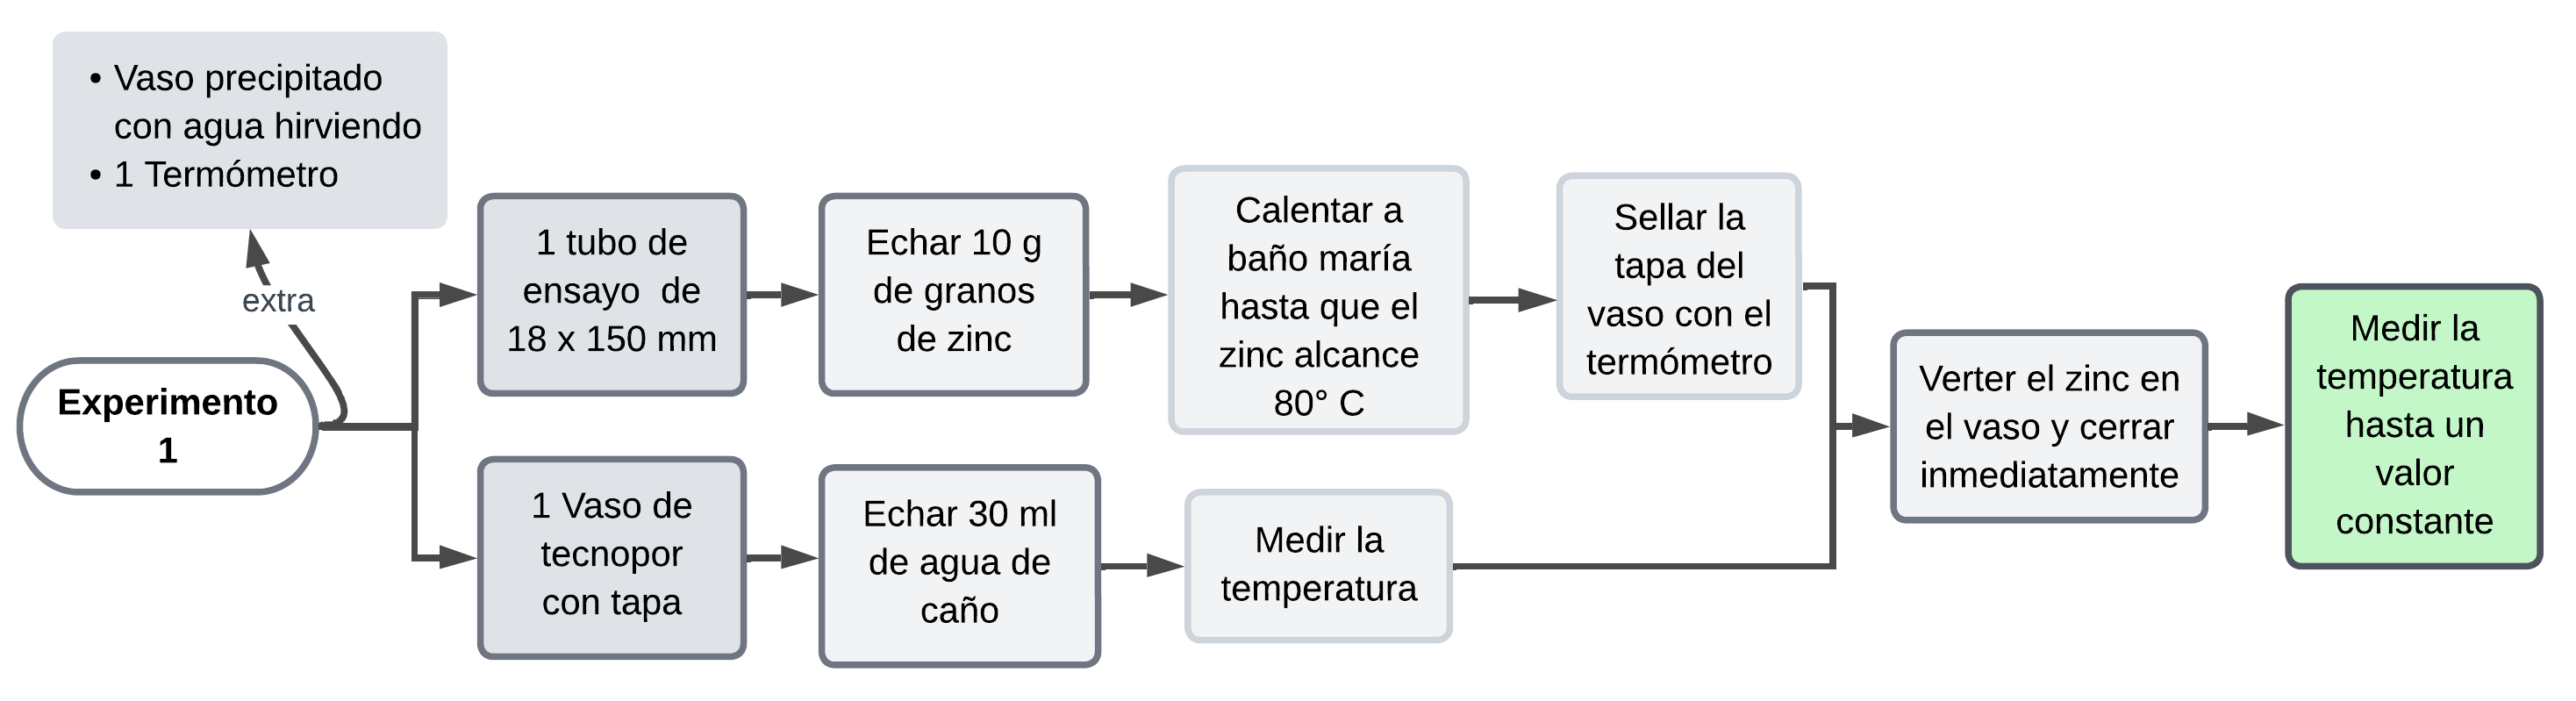
\includegraphics[width = 1\textwidth]{Imagenes/Exp1.png}
	\end{center}
    \end{figure}
    
\subsection{Experimento 2}
    \begin{figure}[H]
	\begin{center}
         \caption{Determinación del calor de neutralización entre el NaOH y el HCl}  {\label{fig:exp2}} 
        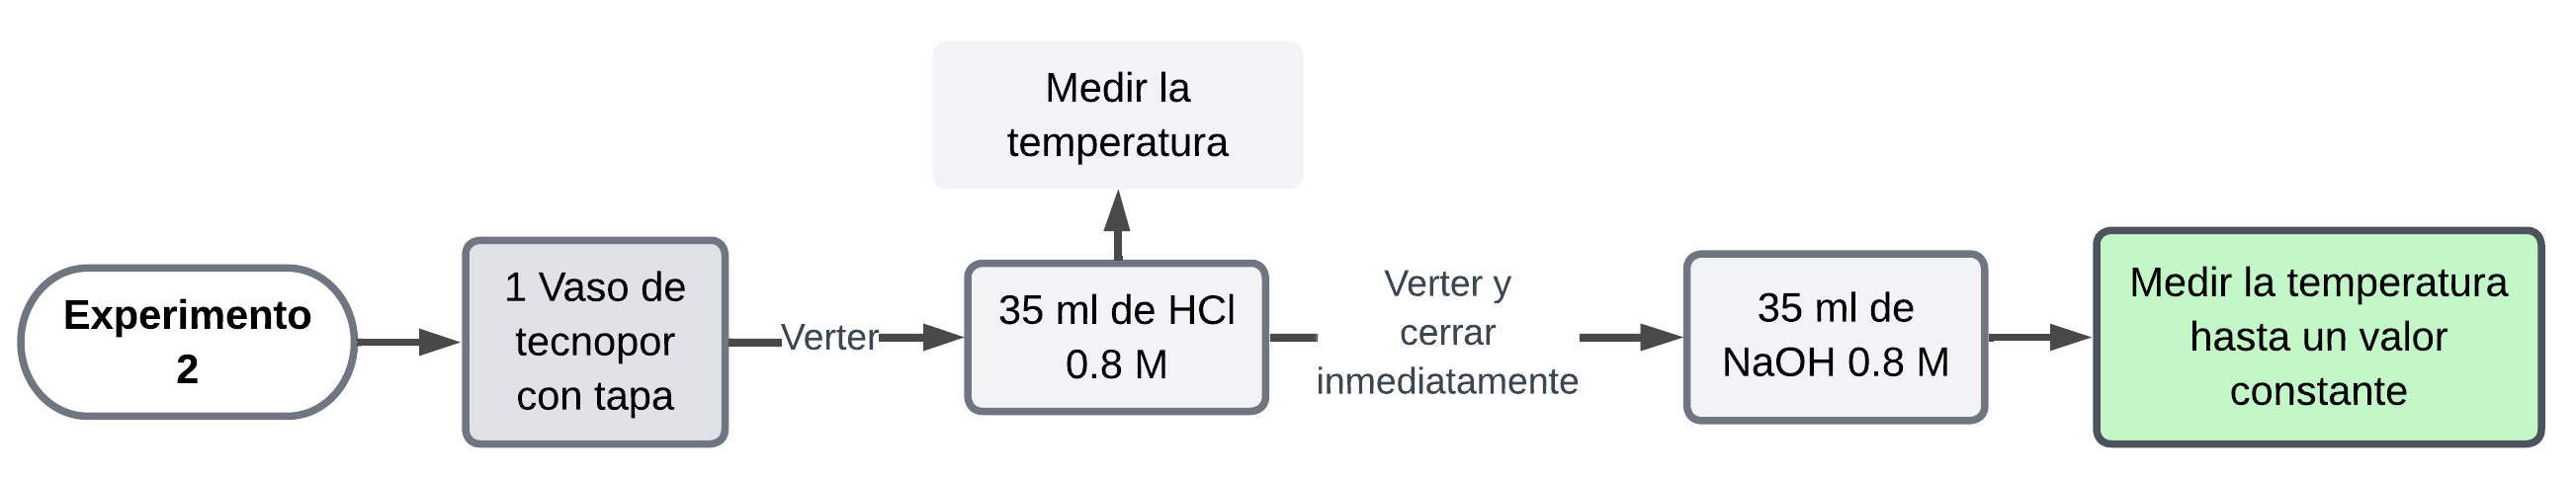
\includegraphics[width = 1\textwidth]{Imagenes/Exp2.png}
	\end{center}
    \end{figure}
    
\subsection{Experimento 3}
    \begin{figure}[H]
	\begin{center}
         \caption{Determinación del calor de disolución del NaCl}  {\label{fig:exp3}} 
        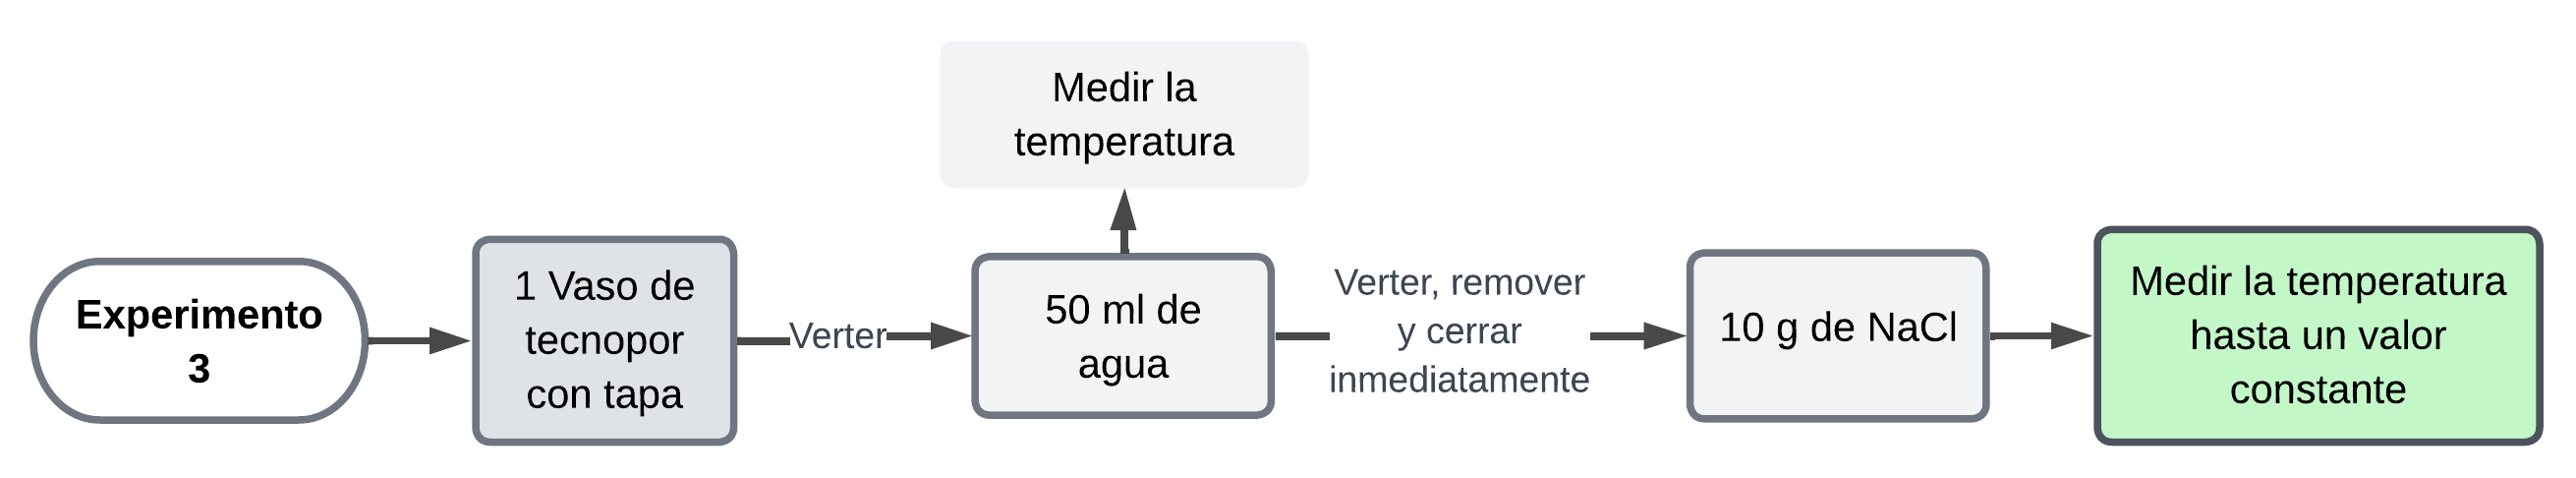
\includegraphics[width = 1\textwidth]{Imagenes/Exp3.png}
	\end{center}
    \end{figure}

\newpage
\section{Datos tabulados}
\subsection{Experimento 1}

\begin{table}[H]
\caption{Datos para la determinación del c.e. del Zinc} \label{tab:zinc}
\centering
\begin{tblr}{
  cells = {c},
  hlines,
  hline{1,3} = {-}{0.15em},
}
{Masa inicial\\ de agua} & {Temperatura\\inicial del H$_{2}$O} & {Masa inicial\\ de Zinc} & {Temperatura\\Zinc caliente} & {Temperatura\\final de la Mezcla} \\
{~\\30 g\\~} & {~\\25 $^\circ$C\\~} & {~\\10 g\\~} & 
{~\\80 $^\circ$C\\~} & {~\\26,5 $^\circ$C\\~}
\end{tblr}
\end{table}

\subsection{Experimento 2}

\begin{table}[H]
\caption{Datos para determinar $\Delta$H de la neutralización de HCl 0,8 M y NaOH 0,8 M} \label{tab:neutra}
\centering
\begin{tblr}{
  cells = {c},
  hlines,
  hline{1,3} = {-}{0.15em},
}
{~Volumen~\\inicial de HCl} & {~Temperatura~\\inicial de HCl} & {~Volumen~\\inicial de NaOH} &{~Temperatura~\\inicial de NaOH} & {Temperatura en\\la neutralización} \\
{~\\35 ml\\~} & {~\\25 $^\circ$C\\~} & {~\\35 ml\\~} &
{~\\25 $^\circ$C\\~} & {~\\29,7 $^\circ$C\\~}\\
\end{tblr}
\end{table}

\subsection{Experimento 3}

\begin{table}[H]
\caption{Datos para determinar $\Delta$H de disolución de NaCl} \label{tab:disolucion}
\centering
\begin{tblr}{
  cells = {c},
  hlines,
  hline{1,3} = {-}{0.15em},
}
{Masa inicial\\ de H$_{2}$O} & {Temperatura\\inicial de H$_{2}$O} & {Masa inicial\\de NaCl} & {Temperatura en la\\ disolución de NaCl}\\
{~\\50 g\\~} & {~\\25 $^\circ$C\\~} & {~\\10 g\\~} &
{~\\23,5 $^\circ$C\\~}\\
\end{tblr}
\end{table}

\section{Observaciones}



\newpage
\section{Cálculos y resultados}

\subsection{Cáculo del calor específico del Zinc}
\vspace{2mm}
\textbf{Uso de los siguientes recursos}
    \begin{itemize}
        \item Datos provistos en el Cuadro \ref{tab:zinc}
        \item Constantes y asunciones:
        \begin{itemize}
            \item C.E. de H$_{2}$O a 25 $^\circ$C = 4,18 J/g-K
            \item El calorímetro usado es ideal, por tanto:\\ 
                    \emph{Q ganado por el agua = Q perdido por el Zinc}
        \end{itemize}
        \item Fórmula:
        \begin{equation}
            m_{H_{2}O}\times C.E._{H_{2}O} \times\Delta T = -(m_{Zn} \times C.E._{Zn} \times\Delta T)
        \end{equation}
    \end{itemize}
\vspace{2mm}
\hspace{0.5cm}\textbf{Cálculos}

\begin{equation*}
            (30)\times(4,18)\times(26,5-25) = -(10)\times (C.E._{Zn})\times(26,5-80)
        \end{equation*}
 \vspace{0.1cm}       
\begin{equation*}
            \frac{(188.1)}{535}=C.E._{Zn}
        \end{equation*}
\vspace{0.1cm}
\begin{equation*}
            0.35=C.E._{Zn}
        \end{equation*}

\begin{center}
    \textbf{El calor específico del Zinc es 0,35 J/g-K}
\end{center}
\enskip
\subsection{Cálculo del calor de neutralización entre NaOH y HCl}
   \vspace{2mm}
\textbf{Uso de los siguientes recursos}
    \begin{itemize}
        \item Datos provistos en el Cuadro \ref{tab:neutra}
        \item Constantes y asunciones:
        \begin{itemize}
            \item C.E. de H$_{2}$O a 25 $^\circ$C = 4,18 J/g-K
            \item La densidad de la solución es 1g/mL
            \item El calorímetro usado es ideal, por tanto:\\ 
                \emph{Q ganado por el agua = Q perdido por el Zinc}\\ \emph{Q solución = - Q neutralización}
        \end{itemize}
        \item Fórmula:
        \begin{equation}
           - ~ \Delta H_{Neutralizaci\acute{o}n} = \frac{m_{H_{2}O} \times C.E._{H_{2}O} \times\Delta T}{n_{\acute{a}cido}} 
        \end{equation}

    \end{itemize}
\vspace{2mm}
\hspace{0.5cm}\textbf{Cálculos}

\begin{equation*}
           - ~ \Delta H = \frac{(70)\times(4,18)\times(29,7-25)}{n_{HCl}}
        \end{equation*}
\vspace{0.1cm}
\begin{equation*}
            n_{HCl} = Moralidad \times Volumen = 0,8 \times 0,035 = 0,028 ~ mol
        \end{equation*}
 \vspace{0.1cm}       
\begin{equation*}
             ~ \Delta H = \frac{1375,22} {0,028}
        \end{equation*}
\vspace{0.1cm}
\begin{equation*}
           \Delta H = - ~ 49,115 kJ/mol
        \end{equation*}
\begin{center}
    \textbf{La $\Delta$ H de neutralización es - 49,115 kJ/mol}
\end{center}

\subsection{Cálculo del calor de disolución de NaCl}

\textbf{Uso de los siguientes recursos}
    \begin{itemize}
        \item Datos provistos en el Cuadro \ref{tab:disolucion}
        \item Constantes y asunciones:
        \begin{itemize}
            \item C.E. de H$_{2}$O a 25 $^\circ$C = 4,18 J/g-K
            \item El calorímetro usado es ideal
        \end{itemize}
        \item Fórmula:
        \begin{equation}
             - ~\Delta H_{Disoluci\acute{o}n} = \frac{m_{H_{2}O} \times C.E._{H_{2}O} \times\Delta T}{n_{sal}}
        \end{equation}
    \end{itemize}

\textbf{Cálculos}

\begin{equation*}
             - ~\Delta H = \frac{(50)\times(4,18)\times(23,2-25)}{n_{NaCl}}
        \end{equation*}
\vspace{0.1cm}
\begin{equation*}
            n_{HCl} = \frac{m_{NaCl}}{m/mol_{NaCl}} = \frac{10}{58.44} = 0,171 ~ mol
        \end{equation*}
 \vspace{0.1cm}       
\begin{equation*}
            - ~\Delta H = -\frac{376,2}{0,171}
        \end{equation*}
\vspace{0.1cm}
\begin{equation*}
           \Delta H = 2,2 kJ/mol
        \end{equation*}
\begin{center}
    \textbf{La $\Delta$ H de neutralización es 2,2 kJ/mol}
\end{center}


\section{Discusión de resultados}
\begin{itemize}
    \item Hubo una diferencia considerable entre el peso ideal de CaCO$_3$ y el resultado experimental, que se puede deber a la perdida de muestra y a la eficiencia de la reacción.
    \item Se evidenció gases debido a la reacción del ácido HCl y la caliza CaCO$_3$, liberando CO$_2$ y H$_2$O gaseosos. Así mismo esta reacción sería la causante de la coloración amarillenta de la solución.
    \item La variación del color del alambre acercado al fuego se debió a la absorción del calor y a la emisión de esta en forma de luz, por ello, aún enfriándose, sigue emitiendo algo de luz.
    \item La separación de la sal de la muestra inicial se dió de forma sencilla debido a que el NaCl es iónico y el agua es un solvente polar
    \item La combustión completa en el mechero dió lugar a una llama no luminosa debido a que no hay residuos de la combustión que permanezcan incandescentes en la llama
\end{itemize}

\section{Conclusiones}
\begin{itemize}
    \item Determinamos la diferencia de temperatura en diferentes puntos de una llama, mostrando un rango que va desde 500°-700° (rojo oscuro) en la base, pasando por 900°-1300° (naranja) en el punto medio y finalmente 700°-900° (rojo naranja) en la punta
    \item Identificamos la información en los diamantes de seguridad de dos compuestos que se nos presentaron en el laboratorio e investigamos sus indicaciones de manejos y precaución
    \item  Logramos determinar el peso y concentración aproximados de los compuestos que conformaban la muestra inicial y que estos eran aproximadamente iguales. Además de verificar que había una diferencia considerable entre los valores teóricos y experimentales. 
\end{itemize}




\section{Bibliografía}
\begin{itemize}
    \item Cedrón J, Landa V, Robles J (2014, julio 25). 1.3.1.- Calor Específico y Capacidad Calorífica. Edu.pe. http://corinto.pucp.edu.pe/quimicageneral/contenido/131-calor-especifico-y-capacidad-calorifica.html
    \item Brown, T. (2004). Estequiometría: cálculos con fórmulas y ecuaciones químicas. En G. Trujano (Ed.), Química: La ciencia central (pp. 113-150). Pearson.
\end{itemize}

\end{document}